\documentclass[11pt,a4paper]{article}

\usepackage[utf8]{inputenc}
\usepackage[T1]{fontenc}
\usepackage[french]{babel}
\usepackage[a4paper,margin=2.5cm]{geometry}
\usepackage{setspace}
\usepackage{parskip}
\usepackage{amsmath,amssymb,amsfonts}
\usepackage{graphicx}
\usepackage{float}
\usepackage{caption}
\usepackage{subcaption}
\usepackage{booktabs}
\usepackage{array}
\usepackage[hidelinks]{hyperref}
\usepackage{xurl}
\usepackage{enumitem}
\usepackage{xcolor}
\usepackage{siunitx}
\usepackage{listings}
\usepackage{fancyhdr}
\usepackage{csquotes}

\setlength{\parindent}{0pt}
\setstretch{1.15}

\pagestyle{fancy}
\fancyhf{}
\lhead{Synthèse}
\rhead{Contrôle du mouvement}
\cfoot{\thepage}

\begin{document}

\title{Synthèse -- Contrôle du mouvement}
\author{}
\date{}
\maketitle

\tableofcontents
\newpage

\section{Introduction au contrôle du mouvement}

\subsection{Concepts}

Le \textbf{contrôle du mouvement} est une branche de l'automatique dédiée à la commande de la \textbf{position}, de la \textbf{vitesse}, de l'\textbf{accélération} ou de la \textbf{force} d'une machine.

Ses objectifs principaux sont la \textbf{précision}, la \textbf{sécurité}, la réduction de l'\textbf{effort de commande} et de la \textbf{consommation d'énergie}, ainsi que la maîtrise du \textit{régime transitoire}.

Une boucle de contrôle du mouvement comprend généralement un \textbf{contrôleur}, des \textbf{actionneurs}, des \textbf{capteurs} et le \textbf{système à piloter}.

\begin{figure}[H]
    \centering
    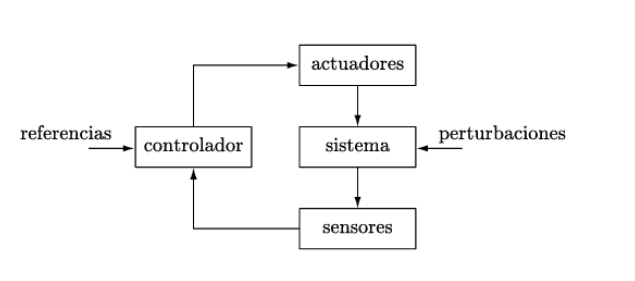
\includegraphics[width=0.7\textwidth]{images/boucle_control.png}
    \caption{Boucle de contrôle}
    \label{fig:boucle_controle}
\end{figure}

\subsection{Technologie}

\subsubsection{Contrôleur}
Le \textbf{contrôleur} est l'unité qui calcule la commande à appliquer au système. Il peut être réalisé à l'aide d'un \textbf{microcontrôleur}, d'un \textbf{automate programmable}, d'un \textbf{DSP} ou d'un \textbf{ordinateur}. Dans certains systèmes, \textit{plusieurs contrôleurs} peuvent être organisés à différents niveaux.

\subsubsection{Actionneurs}
Les \textbf{actionneurs} convertissent la commande en action physique. Les actionneurs \textbf{électriques} sont souvent utilisés pour leur efficacité, les actionneurs \textbf{hydrauliques} pour les fortes charges, et les actionneurs \textbf{pneumatiques} pour des mouvements rapides mais généralement \textit{moins précis}.

\subsubsection{Capteurs}
Les \textbf{capteurs} mesurent les grandeurs nécessaires au contrôle, comme la \textbf{position}, la \textbf{vitesse}, l'\textbf{accélération}, la \textbf{température} ou la \textbf{force}. Ils permettent au contrôleur d'adapter la commande en fonction de l'état réel du système. \textit{Un bon retour de mesure est essentiel pour obtenir un contrôle précis.}


\subsection{Problèmes de contrôle}

\subsubsection{Régulation de consigne}
La \textbf{régulation de consigne} consiste à maintenir le système autour d'une \textbf{référence constante}. L'objectif est d'assurer un comportement stable et de limiter l'effet des perturbations.

\subsubsection{Suivi de trajectoire}
Le \textbf{suivi de trajectoire} consiste à faire évoluer les sorties du système selon une \textbf{référence variable dans le temps}. Il est utilisé lorsque le mouvement doit suivre un profil précis.

\begin{figure}[H]
    \centering
    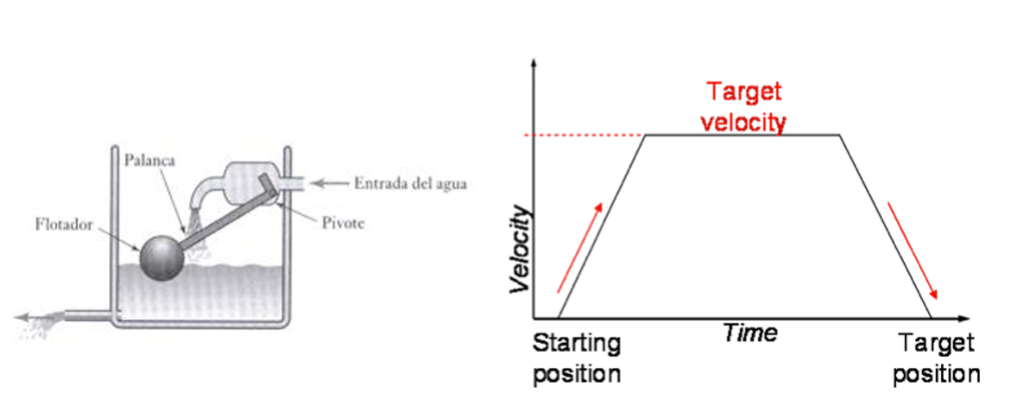
\includegraphics[width=0.7\textwidth]{images/problemas.png}
    \caption{Problèmes de contrôle}
    \label{fig:2}
\end{figure}

\subsection{Champs d'application}

Le contrôle du mouvement apparaît dans de nombreux domaines, notamment dans les \textbf{dispositifs mécatroniques}, la \textbf{robotique} et les \textbf{procédés industriels}.

Parmi les exemples présentés, on peut citer le \textbf{disque dur mécanique}, la \textbf{direction par câble} (\textit{steer-by-wire}), le \textbf{bras robotisé}, le \textbf{robot mobile}, la \textbf{commande numérique par ordinateur} (\textbf{CNC}) et la \textbf{machine d'emballage}.

\newpage
\section{Théorie du contrôle du mouvement}


\subsection{Représentation interne}

\subsubsection{Introduction}

Un \textbf{système}, une \textbf{plante} ou un \textbf{processus} est une entité composée de plusieurs éléments interconnectés, remplissant une fonction déterminée. Ses entrées peuvent être soit des \textbf{variables de commande}, sur lesquelles il est possible d'agir, soit des \textbf{perturbations}, qui influencent le système sans être directement maîtrisées.

Afin d'étudier son comportement, on utilise un \textbf{modèle mathématique}, c'est-à-dire une représentation abstraite du processus réel. Dans de nombreux cas, ce modèle s'exprime à l'aide d'\textbf{équations différentielles}, car elles permettent de décrire l'évolution continue des grandeurs physiques dans le temps.

Par exemple, un système mécanique de type \textit{masse--amortissement--ressort} peut être décrit par :
\[
u = m\ddot{y} + f\dot{y} + qy
\]
où \(u\) représente l'action appliquée au système et \(y\) sa sortie.

\subsubsection{Représentation externe et représentation interne}

La \textbf{représentation externe} décrit directement la relation entre les \textbf{entrées} et les \textbf{sorties} du système, sans modéliser explicitement ce qui se passe à l'intérieur de la plante. Dans ce cadre, l'outil principal est la \textbf{fonction de transfert}, obtenue en appliquant la transformée de Laplace aux équations différentielles du système, sous conditions initiales nulles.

\begin{figure}[H]
    \centering
    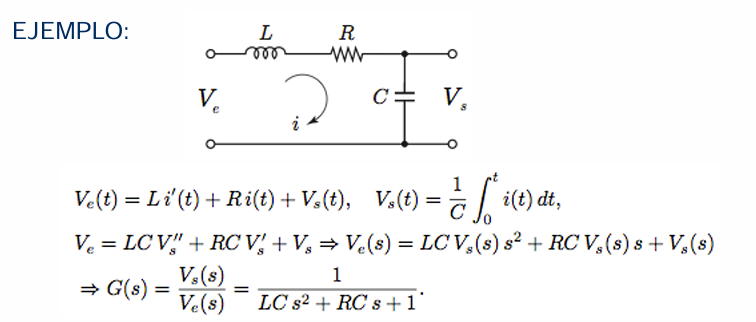
\includegraphics[width=0.7\textwidth]{images/Ej_TF.png}
    \caption{Exemple de fonction de transfert}
    \label{fig:matrice_transfert}
\end{figure}

Dans le cas des systèmes à plusieurs entrées et plusieurs sorties, on utilise une \textbf{matrice de transfert}, qui regroupe les fonctions de transfert reliant chaque entrée à chaque sortie.

\begin{figure}[H]
    \centering
    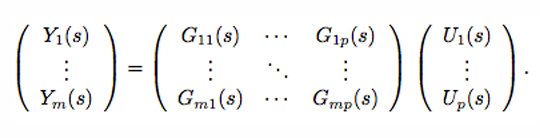
\includegraphics[width=0.5\textwidth]{images/matricedeT.png}
    \caption{Matrice de transfert}
    \label{fig:matrice_transfert}
\end{figure}

La \textbf{représentation interne}, quant à elle, introduit les \textbf{états} du système. Un état est défini comme l'ensemble minimal de variables permettant de résumer le passé du système et de prédire son évolution future. Cette approche permet de décrire plus finement le comportement interne de la plante.

Lorsque cela est possible, il est préférable de choisir des états ayant une \textbf{interprétation physique}, ce qui facilite la compréhension du système.

\subsubsection{Équations d'état et de sortie}

Dans le cas général, la représentation interne d'un système s'écrit sous la forme :
\[
\dot{x}(t)=\phi(x(t),u(t)), \qquad y(t)=\eta(x(t),u(t))
\]
où \(x(t)\) est le \textbf{vecteur d'état}, \(u(t)\) le vecteur des \textbf{entrées} ou des actions, et \(y(t)\) le vecteur des \textbf{sorties}.

\begin{figure}[H]
    \centering
    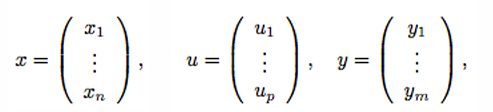
\includegraphics[width=0.5\textwidth]{images/vector.png}
    \caption{Vecteur d'état}
    \label{fig:vector_etat }
\end{figure}

Pour un \textbf{système linéaire invariant dans le temps}, ce modèle devient :
\[
\dot{x}(t)=Ax(t)+Bu(t), \qquad y(t)=Cx(t)+Du(t)
\]

Dans cette écriture :
\begin{itemize}
    \item \(A\) est la \textbf{matrice dynamique} du système. Elle décrit l'évolution \textit{naturelle} des variables d'état en l'absence de commande. Ses coefficients traduisent les couplages entre les états, et ses \textbf{valeurs propres} déterminent en grande partie le comportement dynamique du système, notamment sa rapidité et sa stabilité.

    \item \(B\) est la \textbf{matrice de commande}. Elle indique comment les \textbf{entrées} ou actions \(u(t)\) influencent les variables d'état. Elle décrit donc la manière dont la commande agit sur le système. Si certaines composantes de \(B\) sont nulles, cela signifie que certaines entrées n'agissent pas directement sur certains états.

    \item \(C\) est la \textbf{matrice de sortie}. Elle permet de construire les \textbf{sorties mesurées} à partir des variables d'état. Elle sélectionne ou combine les états qui sont observés en sortie. Ainsi, la sortie ne correspond pas nécessairement à un état unique, mais peut être une combinaison de plusieurs états.

    \item \(D\) est la \textbf{matrice d'influence directe}. Elle représente un effet \textbf{instantané} des entrées sur les sorties, sans passer par la dynamique des états. Dans de nombreux systèmes physiques, cette matrice est nulle, mais elle peut être non nulle lorsque l'entrée agit directement sur la sortie.
\end{itemize}

L'ensemble de tous les états possibles constitue l'\textbf{espace d'état}.

\subsubsection{Lien entre représentation interne et fonction de transfert}

La représentation interne et la représentation externe décrivent un même système sous deux points de vue différents. La première met en avant les \textbf{variables d'état} et la dynamique interne du processus, tandis que la seconde relie directement les \textbf{entrées} aux \textbf{sorties} par l'intermédiaire de la fonction de transfert.

Un point important est que la représentation d'état n'est pas unique. En effet, un \textbf{changement de base} dans l'espace d'état,
\[
\bar{x} = Px \qquad \Rightarrow \qquad x = P^{-1}\bar{x},
\]
avec \(P\) inversible, conduit à une nouvelle écriture du système :
\[
\bar{A} = PAP^{-1}, \qquad \bar{B} = PB, \qquad \bar{C} = CP^{-1}, \qquad \bar{D} = D.
\]
Ainsi, plusieurs descriptions internes peuvent représenter le même système physique. Cependant, ce changement de coordonnées ne modifie pas ses propriétés dynamiques fondamentales.

En particulier, les \textbf{valeurs propres} (autovalores) de la matrice \(A\) sont \textbf{invariantes} par changement de base. Cela signifie que la dynamique propre du système reste la même, même si l'on choisit d'autres variables d'état pour le décrire.

À partir de la représentation interne d'un système linéaire invariant dans le temps,
\[
\dot{x}(t)=Ax(t)+Bu(t), \qquad y(t)=Cx(t)+Du(t),
\]
on peut obtenir directement la \textbf{fonction de transfert} :
\[
G(s)=\frac{Y(s)}{U(s)}=C(sI-A)^{-1}B+D.
\]
Cette relation montre que la description entrée--sortie peut être déduite de la description par états. Autrement dit, la représentation interne est plus générale : elle contient suffisamment d'information pour reconstruire la représentation externe.

Ce résultat permet également de comprendre le lien entre les \textbf{pôles} de la fonction de transfert et les \textbf{autovaleurs} de la matrice \(A\). En effet, le terme \((sI-A)^{-1}\) fait apparaître le déterminant \(\lvert sI-A \rvert\) au dénominateur. Les racines de ce déterminant sont précisément les autoval eurs de \(A\). Elles correspondent donc aux pôles du système, sauf dans certains cas particuliers où des simplifications algébriques peuvent apparaître.

Ainsi, l'étude de la matrice \(A\) dans la représentation interne permet d'accéder directement aux propriétés dynamiques essentielles du système, comme la \textbf{stabilité}, la \textbf{rapidité} ou le \textbf{caractère oscillatoire} de la réponse.

L'exemple du \textbf{circuit RLC} illustre bien ce lien. En choisissant comme états le \textbf{courant} \(x_1=i\) et la \textbf{tension du condensateur} \(x_2=V_s\), on obtient une représentation interne du système. À partir de celle-ci, on retrouve ensuite la fonction de transfert du circuit. Le dénominateur de cette fonction de transfert est identique au polynôme caractéristique de la matrice \(A\), ce qui confirme l'équivalence entre \textbf{pôles} et \textbf{autovaleurs}.

Cette correspondance est fondamentale en automatique, car elle permet de passer naturellement d'une analyse en \textbf{espace d'état} à une analyse en \textbf{fonction de transfert}, selon l'outil le plus adapté au problème étudié.

\begin{figure}[H]
    \centering
    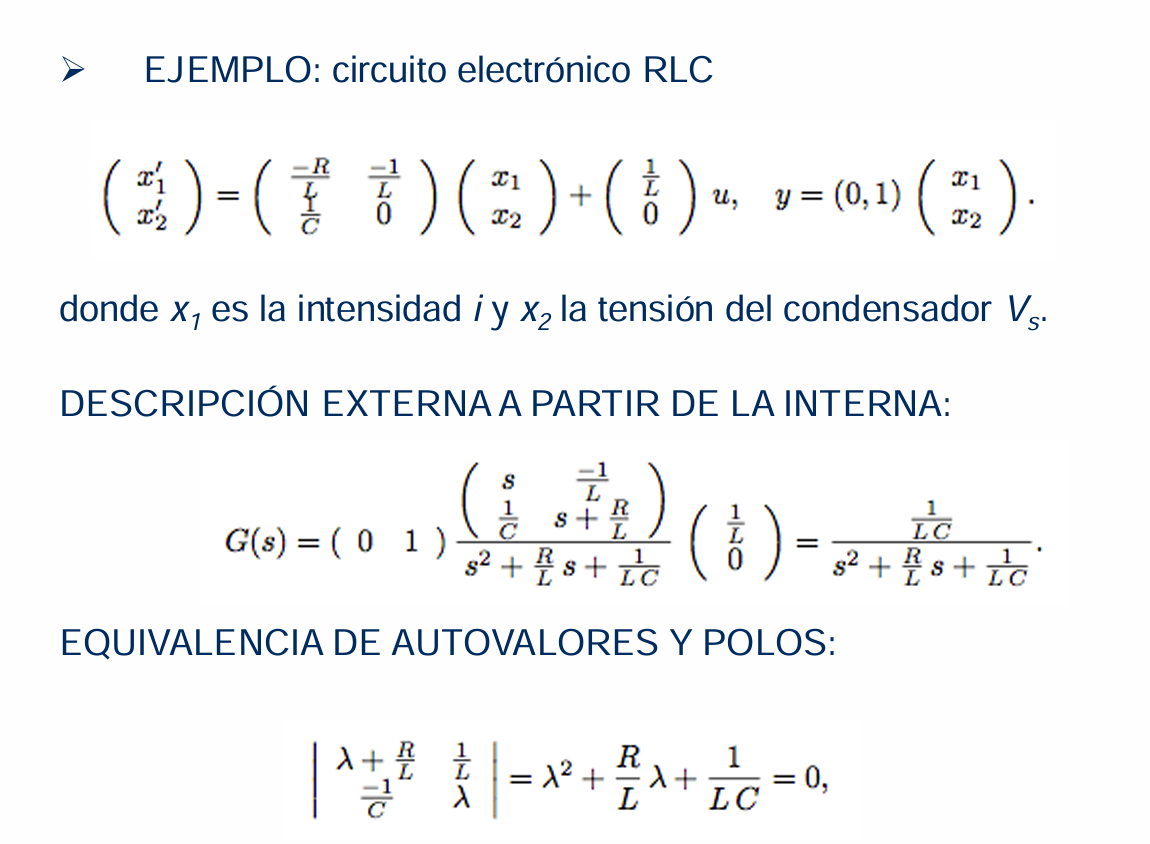
\includegraphics[width=0.8\textwidth]{images/EJ2.png}
    \caption{Exemple du circuit RLC}
    \label{fig:3 }
\end{figure}

\subsubsection{Comparaison entre théorie classique et théorie moderne}

La \textbf{théorie classique du contrôle} repose principalement sur la \textbf{représentation externe}. Elle met l'accent sur le \textbf{signal d'erreur}, défini comme la différence entre la consigne et la sortie mesurée. Cette approche est efficace pour des systèmes simples, mais elle devient moins adaptée lorsque le système est complexe, multivariable ou non linéaire.

La \textbf{théorie moderne du contrôle} repose, au contraire, sur la \textbf{représentation interne}. Elle travaille dans le domaine du temps, avec des outils vectoriels et matriciels. Cette formulation est mieux adaptée à l'étude des systèmes à plusieurs entrées et plusieurs sorties, ainsi qu'aux systèmes non linéaires.

Ainsi, la représentation interne constitue une base essentielle pour l'analyse avancée et la synthèse de lois de commande en contrôle du mouvement.

\subsubsection{Retards de transport}
\subsubsection{Propriétés de la représentation interne}
\subsubsection{États récupérables}

\subsection{Régulation de consignes}

\subsubsection{Principe de la régulation}
\subsubsection{Retour d'état}
\subsubsection{Assignation de pôles}
\subsubsection{Calcul des références}
\subsubsection{Variables d'intégration}
\subsubsection{Cas de plusieurs actionnements}
\subsubsection{Régulation linéaire optimale quadratique}

\subsection{Suivi de trajectoires}

\subsubsection{Définition du problème}
\subsubsection{Schéma général}
\subsubsection{Modèle inverse}
\subsubsection{Variables d'intégration}
\subsubsection{Génération de trajectoires}



\end{document}